\documentclass[12pt]{article}
\usepackage{listings}
\usepackage{color} %red, green, blue, yellow, cyan, magenta, black, white
\definecolor{mygreen}{RGB}{28,172,0} % color values Red, Green, Blue
\definecolor{mylilas}{RGB}{170,55,241}
\usepackage{listings}
\usepackage{qtree}
\usepackage[T1]{fontenc}
\usepackage{indentfirst}
\usepackage{booktabs,amsmath}
\usepackage{amsfonts}
\usepackage[utf8]{inputenc}
\usepackage{amssymb}
\usepackage{graphicx}
\usepackage{xcolor}
\usepackage{float}
\usepackage[bottom]{footmisc}
\usepackage[hidelinks,bookmarks=false]{hyperref}
\usepackage{epstopdf}
\usepackage{enumitem}
\usepackage{xcolor}
\usepackage{multirow}
\usepackage{tabularx}
\usepackage{bbm}
\usepackage{mathtools}
\usepackage{bm}
\usepackage{hyperref}
\usepackage{esvect}
\newcommand\myworries[1]{\textcolor{red}{#1}}
\newcommand\mythoughts[1]{\textcolor{blue}{#1}}
\newcommand\independent{\protect\mathpalette{\protect\independenT}{\perp}}
\def\independenT#1#2{\mathrel{\rlap{$#1#2$}\mkern2mu{#1#2}}}
\usepackage{hyperref}
\usepackage{scalerel,stackengine}
\stackMath
\newcommand\reallywidehat[1]{%
\savestack{\tmpbox}{\stretchto{%
  \scaleto{%
    \scalerel*[\widthof{\ensuremath{#1}}]{\kern-.6pt\bigwedge\kern-.6pt}%
    {\rule[-\textheight/2]{1ex}{\textheight}}%WIDTH-LIMITED BIG WEDGE
  }{\textheight}% 
}{0.5ex}}%
\stackon[1pt]{#1}{\tmpbox}%
}
\parskip 1ex
\hypersetup{
	colorlinks,
	linkcolor={red!50!black},
	citecolor={red!80!black},
	urlcolor={blue!80!black},
	pdfstartview={}
}
\usepackage{dirtytalk}
\newcommand\norm[1]{\left\lVert#1\right\rVert}
\usepackage{lmodern}
\usepackage{booktabs, caption, makecell}
\usepackage{threeparttable}
\usepackage[round, authoryear]{natbib}
\usepackage[left=2.5cm,right=2.5cm,top=2.5cm,bottom=2.5cm]{geometry}
\newtheorem{theorem}{Theorem}
\newtheorem{acknowledgement}{Acknowledgement}
\newtheorem{algorithm}{Algorithm}
\newtheorem{assumption}{Assumption}
\newtheorem{axiom}{Axiom}
\newtheorem{case}{Case}
\newtheorem{claim}{Claim}
\newtheorem{conclusion}{Conclusion}
\newtheorem{condition}{Condition}
\newtheorem{conjecture}{Conjecture}
\newtheorem{corollary}{Corollary}
\newtheorem{criterion}{Criterion}
\newtheorem{definition}{Definition}
\newtheorem{example}{Example}
\newtheorem{exercise}{Exercise}
\newtheorem{lemma}{Lemma}
\newtheorem{notation}{Notation}
\newtheorem{problem}{Problem}
\newtheorem{Proof of Lemma}{Proof of Lemma}
\newtheorem{proposition}{Proposition}
\newtheorem{remark}{Remark}
\newtheorem{solution}{Solution}
\newtheorem{summary}{Summary}
\newenvironment{proof}[1][Proof]{\noindent\textbf{#1.} }{\ \rule{0.5em}{0.5em}}
\bibliographystyle{kluwer}
\usepackage{setspace}

\lstset{basicstyle=\footnotesize\ttfamily,breaklines=true}
\lstset{framextopmargin=50pt,frame=bottomline}

\DeclareMathOperator*{\argmax}{arg\,max}
\DeclareMathOperator*{\argmin}{arg\,min}

\title{Enhancing Glioma Grading with Sparse, Interpretable Classification Models: A Comparative Investigation}
\author{Steven Tang}
\date{November 26, 2024\\}

\usepackage{hyperref}
\usepackage{graphicx}
\usepackage{subfigure}

\begin{document}

\maketitle


\section{Background}
\subsection{Introduction}

Gliomas are tumors arising from glial cells, which nourish, protect, and support neurons in the nervous system. 
There are two grades of glioma: lower-grade gliomas (LGG; grades I and II) and glioblastoma multiforme (GBM), 
a higher grade glioma. In oncology, whereas \textit{stage} describes how much the tumor has spread, \textit{grade} characterizes 
the aggressiveness of the tumor, so GBM is the most aggressive form. The grading of tumor cells involves a wide
range of clinical, histological, and genetic features, and by characterizing the tumor cell’s aggressiveness successfully, 
oncologists and other healthcare workers can effectively determine the quality and course of care, treatment, and prognosis for the 
patient. However, genetic testing for mutations of critical genes can be costly; therefore, it is best if we can find 
a small subset of those genes, coupled with demographic information, that can best characterize a glioma as GBM or LLG. 
In this study, we wish to compare various models exhibiting a wide range of sparsity/interpretability on one facet and predictive 
ability on the other.

\subsection{Data Description}

To investigate this problem, we use the ``Glioma Grading Clinical and Mutations'' dataset from the University 
of California, Irvine (UCI) Machine Learning Repository, derived from the Cancer Genome Atlas (TCGA). 
This dataset encompasses 3 clinical factors (including age, race, and gender) along with 20 binary variables characterizing 
whether the 20 genes associated with each variable are mutated.

There are a total of 839 observations of glioma patients originating from TCGA, 
each with 24 features (described in depth in Table \ref{tab:vars}) and no missing data. We 
first split the data so that 80\% of it is used for training and the rest are held out for testing, as
stratifying so that that class labels are proportionately split. Approximately 57.97\% percent of the 
training data consist of LGG, whereas the other 42.03\% consists of GBM, suggesting mild class imbalance.

Our first step was to plot frequencies of the non-genetic features of the dataset
shown in Figure~\ref{fig:nongenes}. This includes a histogram of the age at diagnosis (in years,
with days in the year forming the decimal part of the data point), the only continuous
feature that we have, as well as bar plots of race and gender. It appears that White patients seem to be disproportionately more 
represented than all other races, followed by Black and African Americans, Asians, and 
American Indians and Alaskan Natives. Additionally, there appears to be more male than 
female patients. The ages appear to be bimodal, with peaks around ages 35 and 65.

Since race is a nominal categorical variable rather than ordinal, we decided to one-hot encode
each level; in other words, each level of race is given its own column, with entries indicating 
whether or not the patient is of that particular race. Due to there being a miniscule 
amount of American Indians and Alaskan Natives, we decide to remove the column; doing so also allows 
for the reduction of redundant information since zero values for each of these other binarized columns for race 
indicate that the patient is indeed American Indian and Native American. Since all of the features
except the age at diagnosis are now binary, we decide to use min-max scaling on the age at diagnosis,
so all variables are between 0 and 1. 

We then look at the mutation counts of various genes in Figure~\ref{fig:genes}. There appears to be as 
many mutated IDH1 and TP53 genes as non-mutated ones. All other genes suggest extreme level imbalance within the 
training dataset, though to a lesser extent for ATRX, PTEN, EGFR, CIC, and MUC16.

The relationships of the mutations of genes and whether or not a glioma is LGG or GBM is of immense interest before 
fitting any classification model. We sample 100 individuals from the dataset, in a manner that corresponds to the class imbalance; we select 58 of them to
be lower-grade glioma patients and the other 42 to be glioblastoma multiforme patients. In Figure~\ref{fig:mutgrid}, we plot whether or not
the given gene is mutated for the patient. There, we notice that LGG patients tend to have more instances of IDH1, TP53, CIC, and ATRX mutated 
compared to GBM patients, where GBM patients tend to have more PTEN and RB1 genes mutated. We then plot a receiver operator characteristic (ROC) curve in
Figure \ref{fig:roc-eda} for 
each feature; each curve then represent the ROC for a predictive model (namely logistic model) involving only the given feature. 
Since almost all of the features are binary, notice that all but the Age curve consists of only two lines; on the other hand, the 
Age curve due to the number of unique values for that feature seems be smoother. Immediately, we see that age, as well as the mutations of IDH1, PTEN,
and ATRX, among others, seem to be the most informative features to consider in a predictive model, aligning well with our observations
about Figure~\ref{fig:mutgrid}.

\begin{figure}[h!]
  \centering
  \subfigure[Age at Diagnosis]{
      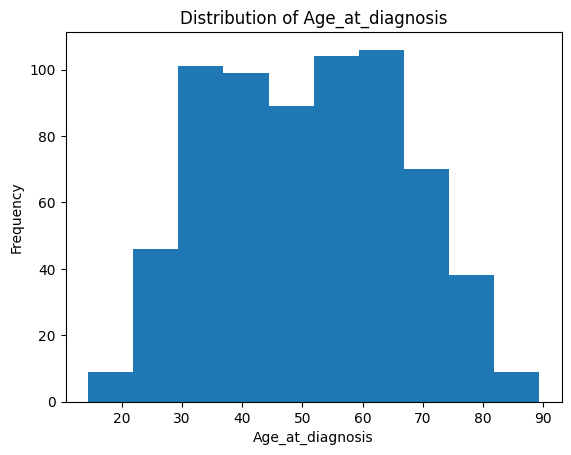
\includegraphics[width=0.3\textwidth]{age-hist.png}
  }
  \subfigure[Race]{
      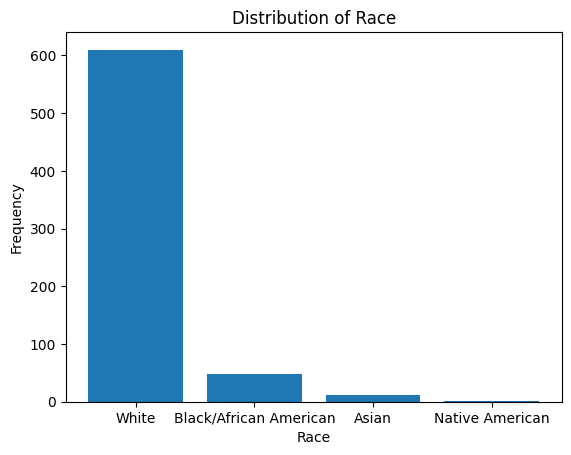
\includegraphics[width=0.3\textwidth]{race.png}
  }
  \subfigure[Gender]{
      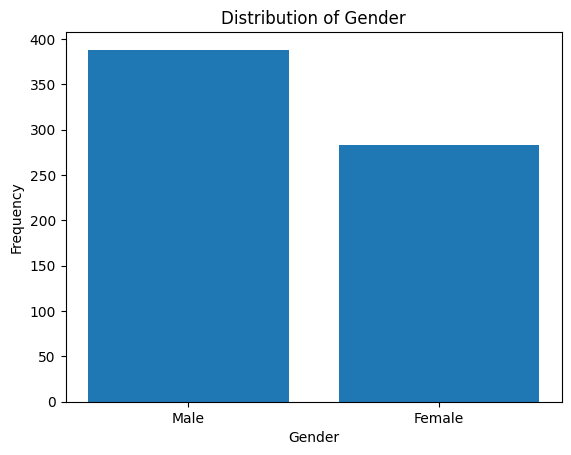
\includegraphics[width=0.3\textwidth]{gender.png}
  }
  \caption{Histograms and barplots of non-genetic features in training data.}
  \label{fig:nongenes}
\end{figure}

\begin{figure}[h!]
  \centering
  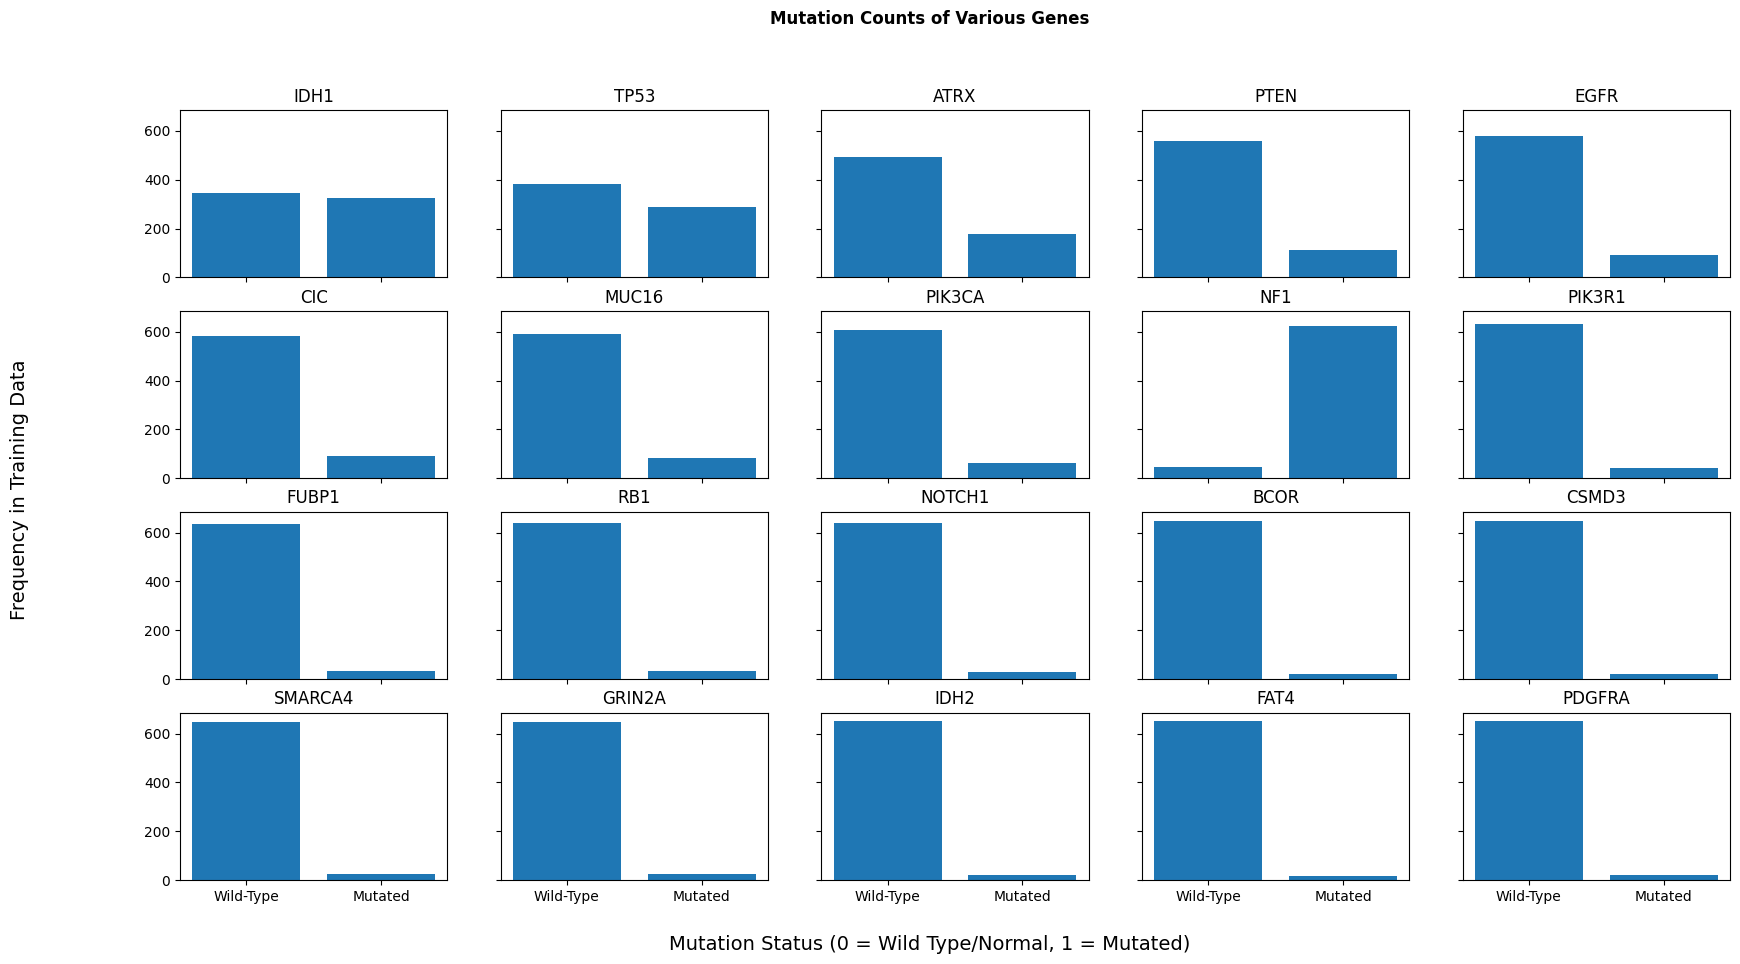
\includegraphics[scale = 0.36]{genes.png}
  \caption{Barplots of Genetic Features in the Training Data}
  \label{fig:genes}
\end{figure}

\begin{figure}[h!]
  \centering
  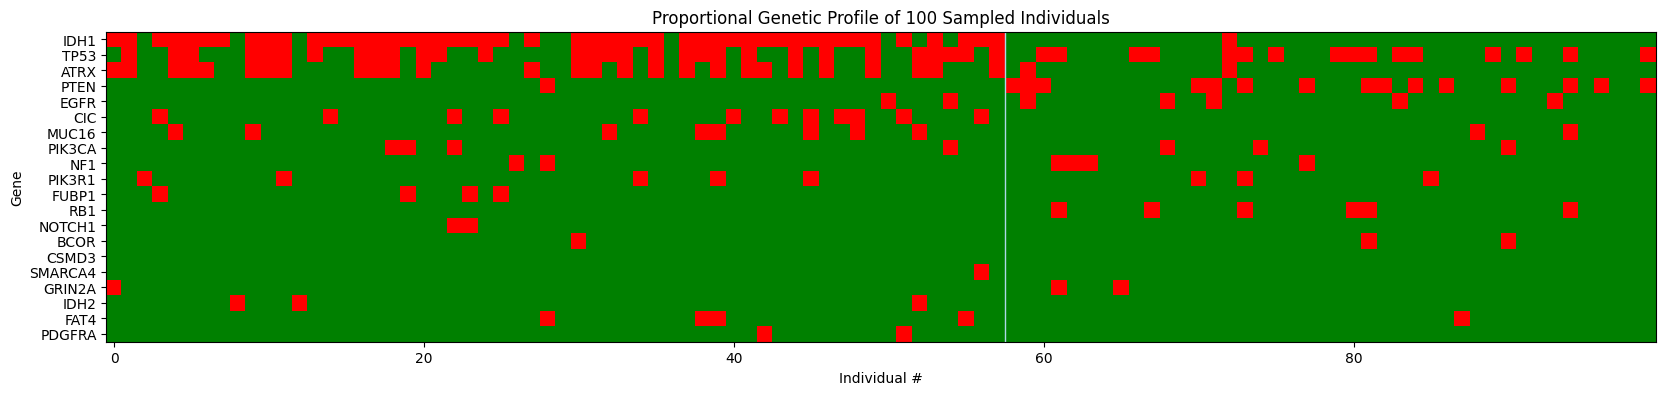
\includegraphics[scale = 0.36]{mutgrid.png}
  \caption{Genetic Profile of 100 individuals (58 LGG patients and 42 GBM patients). The LGG and GBM patients are separated by the faint blue line. Red indicates the mutation of the gene, while green indicates that the gene is normal.}
  \label{fig:mutgrid}
\end{figure}

\begin{figure}[h!]
  \centering
  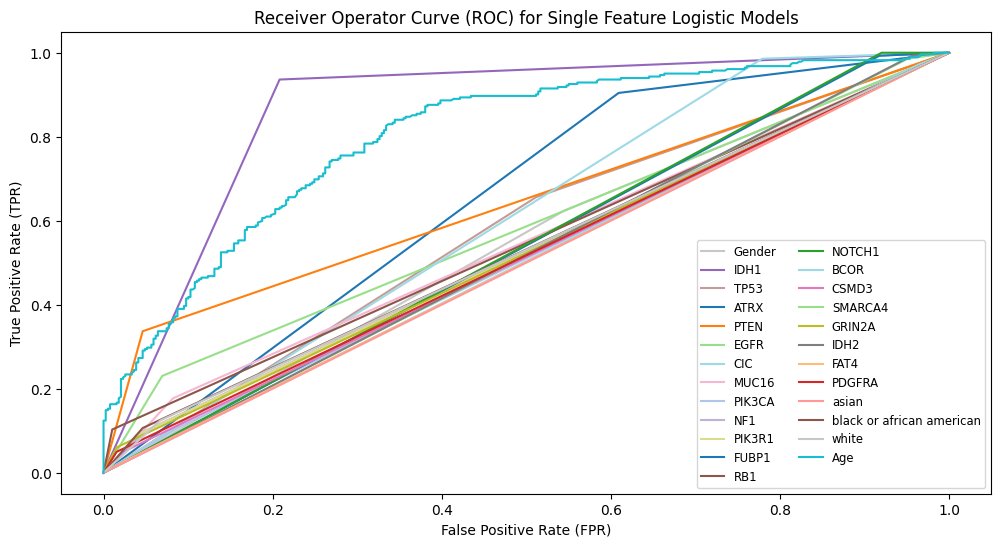
\includegraphics[scale = 0.5]{roc-eda.png}
  \caption{ROC Curves for (dummy) logistic regression models containing only the given feature. }
  \label{fig:roc-eda}
\end{figure}


\begin{table}[h!]
\centering
\caption{Descriptions of the various variables in the TCGA dataset.}
\label{tab:sample_table}
\begin{tabular}{|p{3.5cm}|p{11cm}|p{2cm}|}
  \hline
  \textbf{VARIABLE}         & \textbf{DESCRIPTION} & \textbf{TYPE} \\ \hline
  Grade                     & Glioma Classification (0 = LGG; 1 = GBM)                                                          & Target            \\ \hline 
  Gender                    & Gender (0 = Male; 1 = Female)                                                                     & Binary           \\
  Age\_at\_diagnosis        & Age at diagnosis (in years and days as decimal)                                                   & Continuous       \\
  Race                      & Race\footnotemark(0 = white; 1 = black; 2 = asian; 3 = native)                                    & Categorical      \\ \hline
  IDH1                      & isocitrate dehydrogenase                                                                          & Binary          \\ 
  TP53                      & tumor protein p53                                                                                 & (Genetic\footnotemark)   \\
  ATRX                      & ATRX chromatin remodeler                                                                          & \\
  PTEN                      & phosphotase and tensis homolog                                                                    & \\
  EGFR                      & epidermal growth factor receptor                                                                  & \\
  CIC                       & capicua transcriptional repressor                                                                 & \\
  MUC16                     & mucin 16, cell surface associated                                                                 & \\
  PIK3CA                    & phosphatidylinositol-4,5-bisphosphate 3-kinase catalytic subunit alpha                            & \\
  NF1                       & neurofibromin 1                                                                                   & \\
  PIK3R1                    & phosphoinositide-3-kinase regulatory subunit 1                                                    & \\
  FUBP1                     & far upstream element binding protein 1                                                            & \\
  RB1                       & RB transcriptional corepressor 1                                                                  & \\
  NOTCH1                    & notch receptor 1                                                                                  & \\
  BCOR                      & BCL6 corepressor                                                                                  & \\
  CSMD3                     & CUB and Sushi multiple domains 3                                                                  & \\
  SMARCA4                   & SWI/SNF related, matrix associated, actin dependent regulator of chromatin, subfamily a, member 4 & \\
  GRIN2A                    & glutamate ionotropic receptor NMDA type subunit 2A                                                & \\
  IDH2                      & isocitrate dehydrogenase (NADP(+)) 2                                                              & \\
  FAT4                      & FAT atypical cadherin 4                                                                           & \\
  PDGFRA                    & platelet-derived growth factor receptor alpha                                                     & \\ \hline
  \end{tabular}
  \label{tab:vars}
\end{table}
\footnotetext[1]{For brevity in this table, we use ``black'' for the level ``black and african american'' and ``native'' for ``american indian or alaska native,'' as it appeared in the original data description}
\footnotetext[2]{All genetic binary variables are encoded as wild-type/normal (0) or mutated (1)}
\newpage

\section{Methods}

To build a machine learning model for classifying whether observations associated with patients are lower-grade 
gliomas (LGG) or glioblastoma multiforme (GBM), we use logistic regression with least absolute shrinkage and 
selection operator (LASSO); decision trees; AdaBoost; Random Forests; and FastSparse generalized additive models (GAMs). We opt to use balanced accuracy 
as a metric for model comparison. We use Scikit-learn to fit $L_1$-penalized logistic regression, decision trees, AdaBoost,
and random forest models, and the FastSparseGAMs package to fit FastSparse GAMs. 

\subsection{Classification Algorithms}
\subsubsection{Common (Scikit-Learn) Classification Algorithms}
\textbf{Logistic regression} attempts to predict the log-odds ($\ln\frac{\mathbb{P}(Y=1)}{\mathbb{P}(Y=0)}$) from a linear combination
of the features. We utilize LASSO so that we incorporate an $L_1$-penalty which regularizes the model, shrinking the coefficients 
to zero, so the model can perform feature selection. In doing so, we can end up with an interpretable, sparse model and reduce the 
potential of overfitting, doing so with low computational cost. However, logistic regression makes strong assumptions about the data, 
that the log-odds ratio is linear and that multicollinearity between predictors does not exist or is minimal. 

\textbf{Decision Trees} are interpretable and intuitive, especially in the medical context due to the extensive use of
boolean logic stemming from the decision rules that make up the tree. From the training data, the 
Classification and Regression Tree (CART) algorithm learns a series of decision rules (in tree form) that predict the 
target variable. The computational problem of finding the optimal decision tree is NP-complete, and the CART algorithm
is greedy, only making locally optimal steps. In doing so, the decision tree found may not be the most optimal. Furthermore,
the decisions tree could be unnecessarily complicated (having high depth to model simple concepts, like a diagonal boundary)
due to there being rough transitions, and it is sensitive to small variations in data. Fortunately, decision trees allow for 
pruning to mitigate at least some of these ill-effects. 

To mitigate the risk of overfitting and improve generalizability and robustness, we decide to investigate to ensemble methods,
namely AdaBoost and random forests, a boosting and bagging algorithm, respectively. 

\textbf{AdaBoost} combines 
a sequence of weak learner (each of which does slightly better than random guessing) in such a way that, any subsequent weak learner does better at 
what the previous ones miss. It does so by reweighting the data so that incorrectly predicted observation are weighted higher and 
weak learning algorithm is reapplied, and then placing weights on each of those weak learner. Unfortunately, AdaBoost can be sensitive to 
outliers (always focusing on difficult to predict observations), overfit if the base model is complex, potentially focus more on the minority 
class when there is an imbalance in classes, be computationally expensive to perform, and lack interpretability. 
In using AdaBoost, we may trade off interpretability for predictive ability. 

\textbf{Random forests}, on the other hand, incorporates two sources of randomness to improve generalizability. First, it takes a bootstrap sample of 
the training data, building independent trees in parallel on each. Second, when deciding on a feature to split, it chooses a random subset of a particular
size. Additionally, though the combination of various decision trees through the averaging of predicted probabilities may obscure and remove any sense of 
interpretability, random forests do offer some notion of it with feature importance. However, random forests can be quite computationally expensive to fit.
To limit the complexity of the trees that may be grown, we focus on 3 hyperparameters, namely the number of estimators (trees to grow), the maximum number of 
samples, and the maximum number of features to select.  

In each of the previous classification algorithms, we use grid search with stratified 5-fold cross validation to tune the aforementioned hyperparameters (we describe the parameter setting ). 

\subsubsection{Novel Classification Algorithms}
Finally, \textbf{FastSparseGAMs} (Liu et al. 2022) fits sparse generalized additive models on the training data. Recall that GAMs consist of sums of a nonlinear function application on each feature,
and it has a close connection with Adaboost, in that the decision stumps can be rearranged and added together according to their weights. The FastSparse algorithm works similarly,
but does so with a different objective function (utilizing $L_0$-penalty, a penalty on the number of nonzero coefficients).
It offers immense interpretability in the form of shape functions. The lack of continuous variables and abundence of binary variables is still suitable for use of FastSparseGAM, but 
the shape function that may arise may be dull. Additionally generalized additive models do not assume interactions between features, as opposed to decision trees which do. 
The algorithm requires binarizing the continuous ``Age'' feature. 

Overall, we have a set of algorithms that fit models that differ in interpretability and predictability. With decision trees, logistic regression with LASSO, and FastSparseGAMs, interpretability
is stressed more when compared to algorithms built to reduce overfitting and improve generalizability like AdaBoost and random forests. 

\subsection{Metrics}

We opted in this investigation to use \textit{balanced accuracy}: \[\text{Balanced-Accuracy} = \frac{1}{2}(\text{Sensitivity} + \text{Specificity}) = \frac{1}{2}\Bigg(\frac{TP}{TP + FN}+\frac{TN}{FP + TN}\Bigg)\] 
In various healthcare contexts like our setting, specificity and sensitivity is commonly used. On the one hand, sensitivity asks, what percent of the GBM instances were correctly classified as GBM? This is the same 
as recall in classification tasks. On the other hand, specificity quantifies what the of LGG instances that were classified as LGG; this is the probabilistic complement of the false positive rate, i.e. of all of the 
LGG instances, how many of them were incorrectly predicted as being GBM. Both specificity and sensitivity is crucial as misclassification of an instance of either LGG or GBM may lead to poor prognoses or expensive care.
For example, it is generally harder and more expensive to treat GBM than LGG, and GBM is more aggressive. Incorrect grading may thus lead to worsening of condition if a patient actually had GBM, or a treatment that may 
not be effective and is more expensive than necessary if the patient actually had LGG. Considering these questions, it makes sense we adopt the metric that combines these two measures into one unified metric. 

\section{Experiments}

As stated previously, we performed a stratified split on the whole data, so 80\% of it would be used for training and the other 20\% 
for testing. Utilizing the best hyperparameter settings as described below, we refit the training data using and evaluated it on the held-out test set. 

%On the other hand, we tune the FastSparseGAM algorithm less rigorously. We first fit on the training data, yielding various models incorporating 
%different $L_0$-regularization parameters. For each of those, the model we arrive at is the one report the balanced accuracy for. 
%With regards to the plot showing how balanced accuracy changes with the regularization parameter, we plot relationship between the parameter and the
%balanced accuracy on the test set. 

\subsection{Results}
Based on the balanced accuracy, random forest appears to perform the best (0.862), followed by logistic regression with LASSO and Decision Tree (0.853), and finally
AdaBoost. We see that the model also very noticeably outperforms all others in their receiver-operator characteristic (ROC) curves and thereby their AUCs. 
Logistic regression with LASSO and decision trees give the greatest interpretability compared to the other model; in fact we easily display them in Table~\ref{tab:coefs} and 
Figure~\ref{fig:dtree}. Meanwhile, random forests perform the best but it suffers in interpretability. 

\begin{table}[h!]
  \centering
  \caption{The optimal hyperparameter setting and their associated balanced accuracy on the test set.}
  \begin{tabular}{|c|c|c|}
    \hline
    \textbf{Classification Algorithm}         & \textbf{Hyperparameter Setting} & \textbf{Balanced Accuracy} \\ \hline
    FastSparseGAM & $l_0=1.613$ & 0.862 \\ \hline
    Random Forest & max\_depth = 8 & 0.862 \\
    & max\_features = 25 & \\
    & max\_samples = 167 & \\
    & n\_estimators = 128 &  \\ \hline 
    Logistic Regression (LASSO) & $C = 1$ (default) & 0.853 \\ \hline
    Decision Tree & ccp\_alpha $ = 0.0001$ & 0.853 \\ 
     & max\_depth $ = 4$ & \\
     & max\_leaf\_nodes $ = 16$ & \\ \hline
    AdaBoost & learning\_rate = 0.1 & 0.846 \\
    & n\_estimators = 512 & \\ \hline 
  \end{tabular}
  \label{tab:results}
  \end{table}

However, based on the balance accuracy, FastSparse generalized additive models have the same balanced accuracy; however, the result should taken with caution since it was 
tuned less rigorously. Notwithstanding the lack of rigor in this result, it does demonstrate its competitiveness with other models, including random forests.
More, as can be see in Figure~\ref{fig:shape}, the model is highly interpretable compared to the others. 
\begin{table}[h!]
  \centering
  \caption{The coefficients for logistic regression with LASSO model trained on all of the training data.}
  \begin{tabular}{|c|c||c|c|}
    \hline
    Feature &	Coefficients & Feature & Coefficients\\ \hline
    IDH1    &	-4.01 & PDGFRA  &	0.0 \\ 
    IDH2    &	-2.63 & PIK3CA  &	0.0 \\ 
    NOTCH1  &	-1.74 & BCOR &	0.0\\ 
    NF1     &	-0.86 & black... &	0.28\\
    EGFR    &	-0.60 & RB1 &	0.33 \\
    CIC     &	-0.54 & MUC16 &	0.38 \\ 
    SMARCA4 &	-0.29 & CSMD3	& 0.58\\
    Gender  &	-0.17 & PTEN	& 0.69\\ 
    asian   &	0.0  & GRIN2A &	0.77\\ 
    ATRX    &	0.0 & TP53 &	0.88\\ 
    FAT4    &	0.0 & PIK3R1 &	1.23\\ 
    FUBP1   &	0.0 & Age & 2.03\\
    white   &	0.0 & & \\ \hline
  \end{tabular}
  \label{tab:coefs}
  \end{table}

  \begin{figure}[h!]
    \centering
    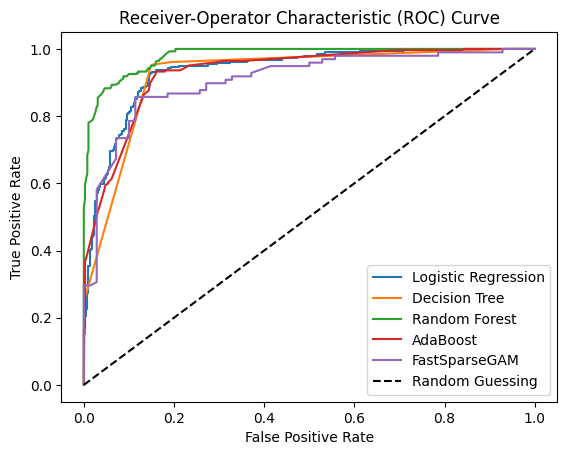
\includegraphics[scale = 1]{roc-results.png}
    \caption{ROC Curves for all models considered. }
    \label{fig:roc-results}
  \end{figure}
\newpage 

\subsection{Hyperparameter Selection}

\begin{table}[h!]
  \centering
  \caption{The hyperparameters used for grid search for each classification algorithm.}
  \begin{tabular}{|c|c|c|}
    \hline
    \textbf{Algorithm} & \textbf{Hyperparameter} & \textbf{Values} \\ \hline
    %FastSparseGAM & $l_0=1.613$ & [168.991, 167.301, 78.474, 62.779, 50.223, 40.179, 32.143, 25.714, 20.571, 16.457, 15.963, 12.771, 10.217, 8.173, 6.539, 5.231, 4.185, 3.348, 3.247, 2.598, 2.078, 2.016, 1.613, 1.564, 1.252, 1.001, 0.971, 0.777, 0.622, 0.603, 0.482, 0.468, 0.454, 0.363, 0.352, 0.282, 0.273, 0.219, 0.212, 0.17, 0.136, 0.132, 0.105, 0.084, 0.067, 0.065, 0.052, 0.051, 0.049, 0.039, 0.031, 0.031, 0.03, 0.024, 0.019, 0.018]    \\ \hline
    Logistic Regression & C & [0.01, 0.025, 0.05, 0.1, 0.5, 1] \\ \hline
    Decision Tree & max\_dept &  [1, 2, 4, 8, 16] \\
    & max\_leaf\_nodes & [2, 4, 8, 16, 32] \\
    & ccp\_alpha & [0.0001, 0.005, 0.01, 0.05, 0.1] \\ \hline
    AdaBoost & learning\_rate & [0.001, 0.005, 0.01, 0.05, 0.1, 0.5, 1] \\
    & n\_estimators & [1, 2, 4, 8, 16, 32, 64, 128, 256, 512] \\ \hline 
    Random Forest & max\_features & [1, 5, 10, 15, 20, 25] \\
    & max\_samples & [335, 167, 83, 41] ($(\lfloor\frac{n}{2}\rfloor, \lfloor\frac{n}{4}\rfloor, \lfloor\frac{n}{8}\rfloor,\lfloor\frac{n}{16}\rfloor)$) \\
    & n\_estimators & [1, 2, 4, 8, 16, 32, 64, 128, 256] \\
    & max\_depth & [1, 2, 4, 8, 16] \\ \hline
  \end{tabular}
  \label{tab:hyperparams}
  \end{table}

Table~\ref{tab:hyperparams} shows the hyperparameter grids we used to perform grid search
for each classification algorithm. For each of the classification algorithms, we performed a grid search on hyperparameters (listed in the Table) utilizing 
stratified 5-fold cross validation to tune the algorithms to find the hyperparameter combination that yielded the greatest balanced accuracy. In order to see how 
each hyperparameter affected the balanced accuracy score, we graph the score by a single hyperparameter while holding all other constant; again, 
this is in contrast to how grid search was used to find the optimal hyperparameter setting. 

\subsubsection{Logistic Regression with LASSO}

For logistic regression, the regularization parameter $C$ was tuned; more regularization is applied with smaller values of $C$. 
Regularization is achieved by putting greater weight on the $L_1$-penalty term. In Figure~\ref{fig:logistic-reg}, we see that the 
less regularization there is, the greater the average balanced accuracy on folds of the training set.

\begin{figure}[h!]
  \centering
  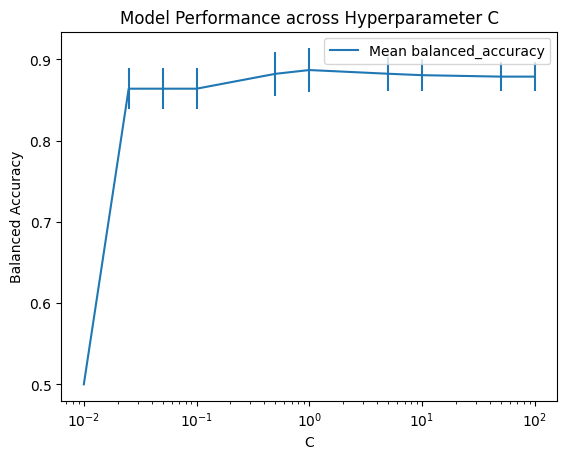
\includegraphics[scale = 0.5]{logisticLASSO-C-param.png}
  \caption{How model performance changes with $\log C$}
  \label{fig:logistic-reg}
\end{figure}

\subsubsection{Decision Tree}

Three parameters are tuned for the CART algorithm to build decision trees according to the training data.
Sparsity and potential for overfitting in a decision tree can depend on the depth of the tree and number of leaves, among other 
hyperparameters. We therefore decide to tune the maximum depth, maximum number of leaf nodes, and the cost-complexity pruning parameter $\alpha$.
Holding all other hyperparameters constant, performance seems to drop off after a maximum depth of 4, maximum number of leaf nodes of 5, 
and cost-complexity pruning parameter of approximately 0.01, as shown in Figure~\ref{fig:dtree}. The maximum depth and cost-complexity pruning 
parameter seem to be effect at improving the model's balanced accuracy. 

\begin{figure}[h!]
  \centering
  \subfigure[Maximum depth]{
      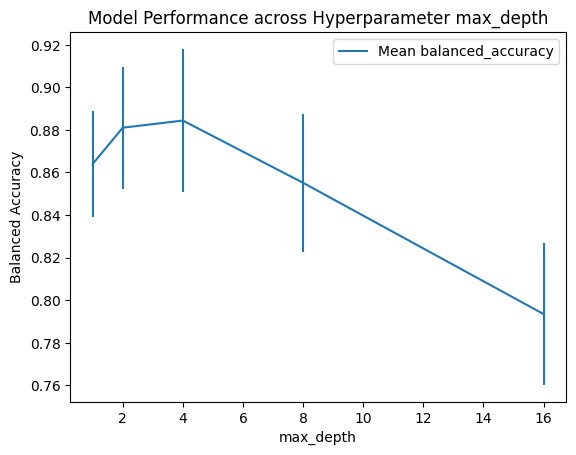
\includegraphics[width=0.3\textwidth]{dtree-maxdepth.png}
  }
  \subfigure[Maximum number of leaf nodes]{
      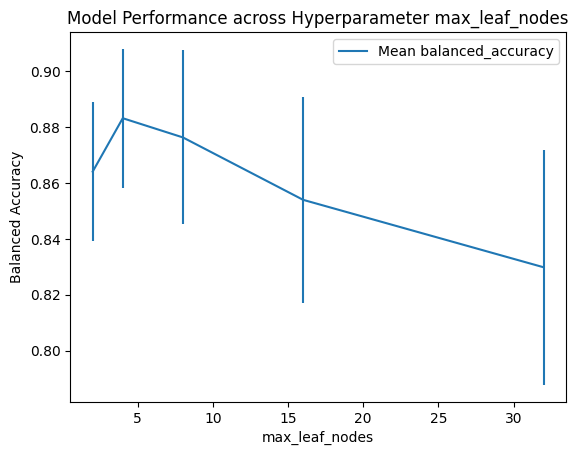
\includegraphics[width=0.3\textwidth]{dtree-maxleafnodes.png}
  }
  \subfigure[Cost-Complexity Pruning Parameter]{
      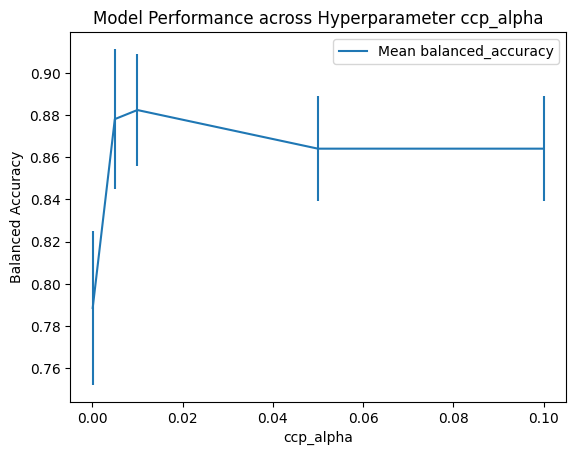
\includegraphics[width=0.3\textwidth]{dtree-ccpalpha.png}
  }
  \caption{How model performance changes with various decision tree hyperparameters (holding every other hyperparameter constant).}
  \label{fig:dtree}
\end{figure}

\subsubsection{AdaBoost}
For the AdaBoost algorithm, we consider a weak learner that is a decision tree of maximum depth 1 (a stump), as well as hyperparameters 
such as the number of estimators and the learning rate. As shown in Figure~\ref{fig:adaboost}, performance peaks around a learning rate of 0.5
and the utilization of 256 estimators. These dynamics are all within a single 
standard deviation of one another. 

\begin{figure}[h!]
  \centering
  \subfigure[Maximum depth]{
      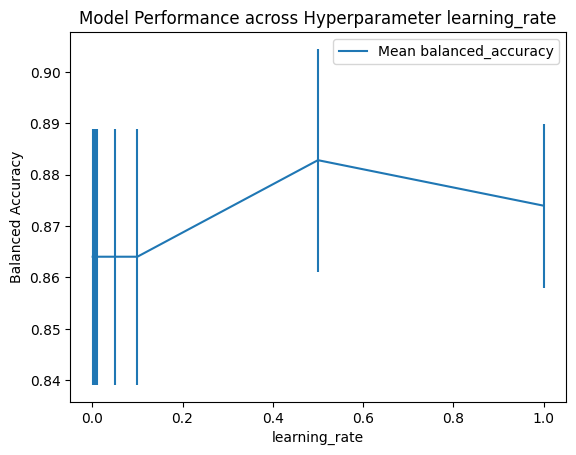
\includegraphics[width=0.4\textwidth]{adaboost-lr.png}
  }
  \subfigure[Maximum number of leaf nodes]{
      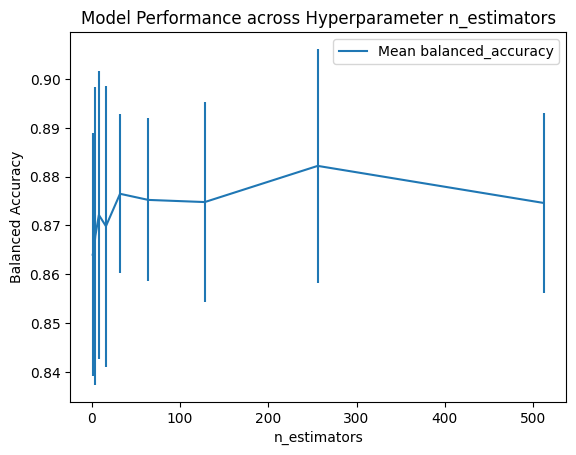
\includegraphics[width=0.4\textwidth]{adaboost-nestimators.png}
  }
  \caption{How model performance changes with various AdaBoost hyperparameters (holding every other hyperparameter constant).}
  \label{fig:adaboost}
\end{figure}

\subsubsection{Random Forest}
For the random forest algorithm, we consider four hyperparameter, common to both decision trees and the AdaBoost algorithm. 
Model performance, according to Figure~\ref{fig:rf} appears to drop off after a max depth of 4; stay constant over the maximum number of features,
though maximized around 5 features; slightly decreases with maximum number of bootstrap samples. These dynamics are all within a single 
standard deviation of one another. 

\begin{figure}[h!]
  \centering
  \subfigure[Maximum depth]{
      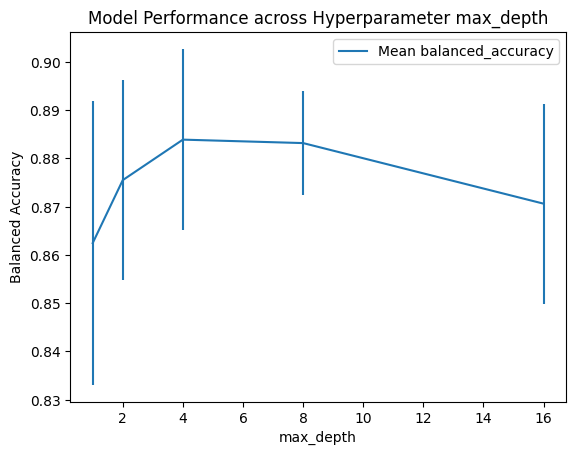
\includegraphics[width=0.4\textwidth]{rf-maxdepth.png}
  }
  \subfigure[Maximum number of features]{
      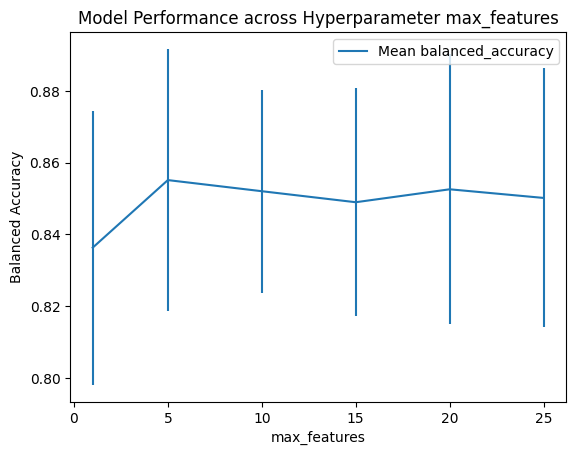
\includegraphics[width=0.4\textwidth]{rf-maxfeatures.png}
  }
  \subfigure[Maximum number of samples]{
      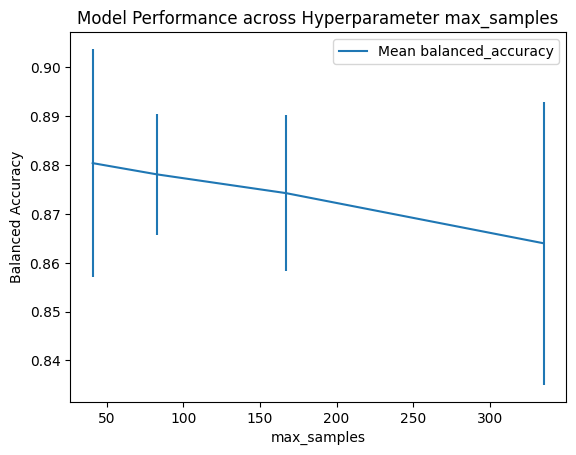
\includegraphics[width=0.4\textwidth]{rf-maxsamples.png}
  }
  \subfigure[Number of Estimators]{
      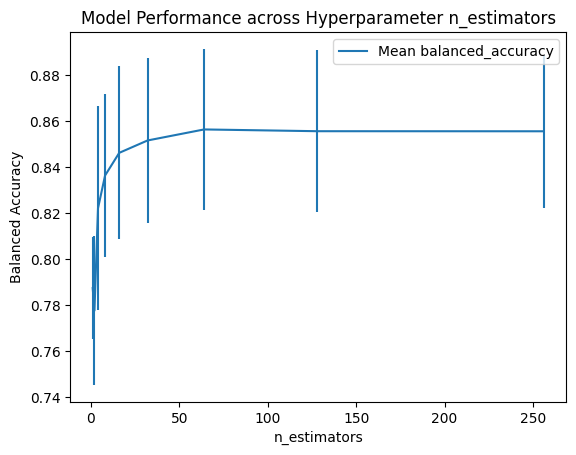
\includegraphics[width=0.4\textwidth]{rf-nestimators.png}
  }
  \caption{How model performance changes with various decision tree hyperparameters (holding every other hyperparameter constant).}
  \label{fig:rf}
\end{figure}
 
\subsubsection{FastSparseGAMs}
For the FastSparseGAM algorithm, we consider a single hyperparameter for the regularization of the $\ell_0$-norm term.
Model performance, according to Figure~\ref{fig:fsg} appears to stay fairly constant across $\log\lambda_0$ but it drops to 0.5 for large values.
\begin{figure}[h!]
  \centering
  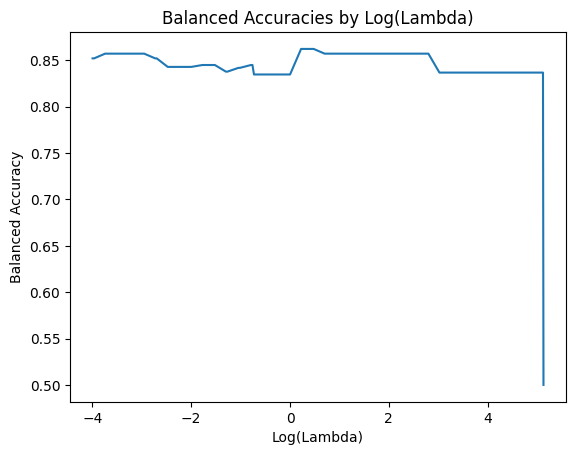
\includegraphics[scale = 0.5]{fsg.png}
  \caption{How model performance changes with $\log \ell_0$}
  \label{fig:fsg}
\end{figure}

\subsection{Variable Importance Analysis}

Below we plot the model reliance of each model; in other words, we permute each 
feature and plot the change in model score from the permutated and original datset.
This measure gives how important a feature is to a the given model. We do so with the
model trained on the whole data. Notice the great similarity between each of the models;
namely it appears that IDH1, IDH2, NOTCH1, and Age all appear to be critical in predicting 
whether a tumor should be graded as GBM or LGG.

\begin{figure}[h!]
  \centering
  \subfigure[Logistic Regression (With LASSO)]{
      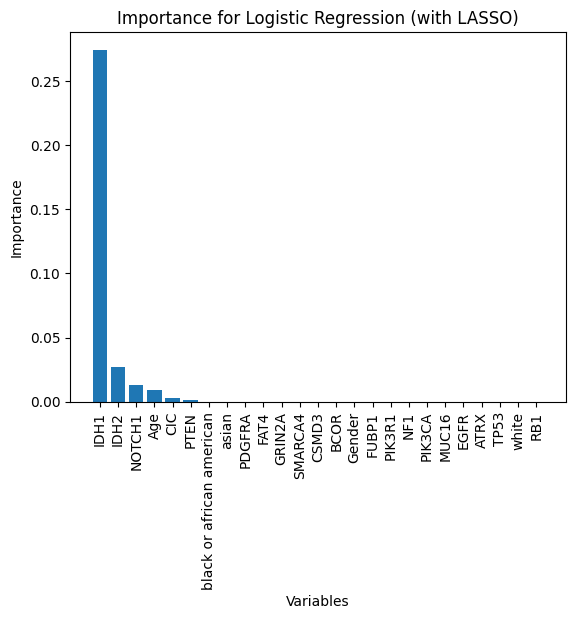
\includegraphics[width=0.4\textwidth]{VI-logistic.png}
  }
  \subfigure[Decision Tree]{
      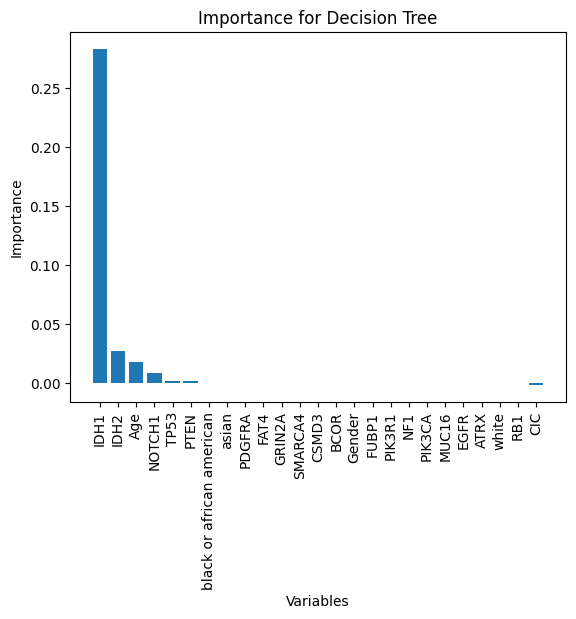
\includegraphics[width=0.4\textwidth]{VI-decisiontree.png}
  }
  \subfigure[AdaBoost]{
      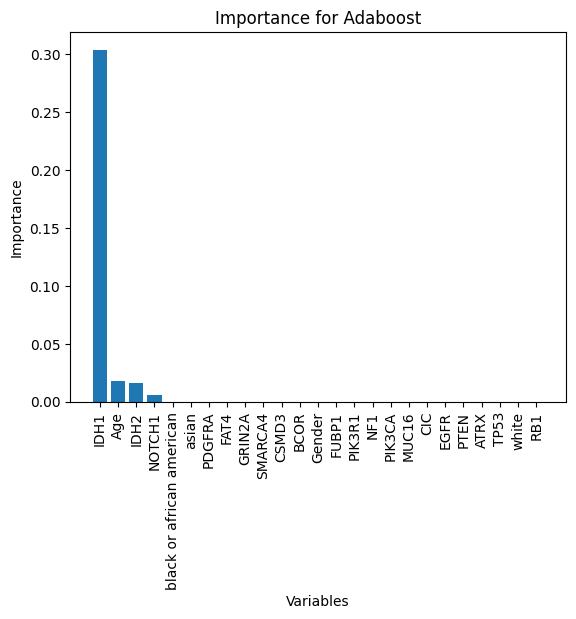
\includegraphics[width=0.4\textwidth]{VI-adaboost.png}
  }
  \subfigure[Random Forest]{
      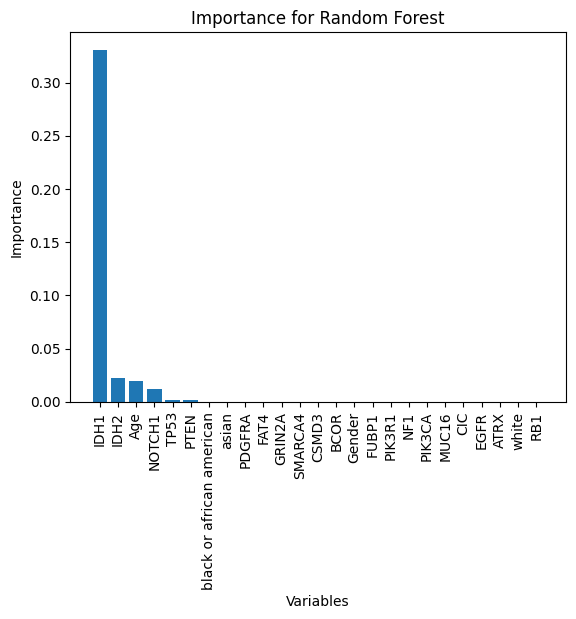
\includegraphics[width=0.4\textwidth]{vi-randomforest.png}
  }
  \caption{Variable Importances (Model Reliance) for each model.}
  \label{fig:vi}
\end{figure}

\begin{figure}[h!]
  \centering
  \subfigure[Age]{
      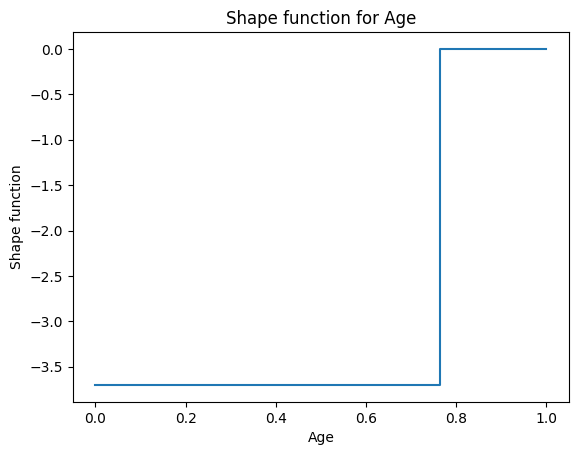
\includegraphics[width=0.3\textwidth]{age-shape.png}
  }
  \subfigure[IDH1]{
      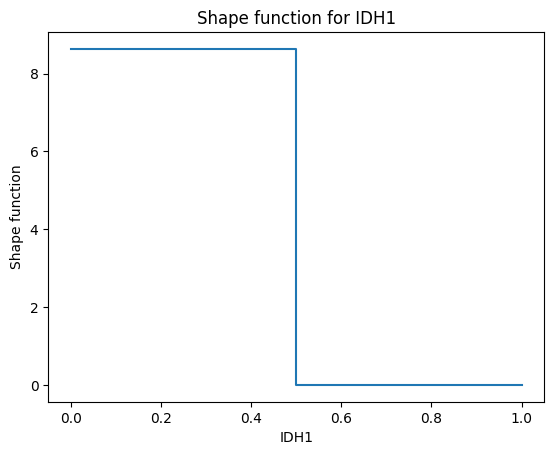
\includegraphics[width=0.3\textwidth]{idh1-shape.png}
  }
  \subfigure[IDH2]{
      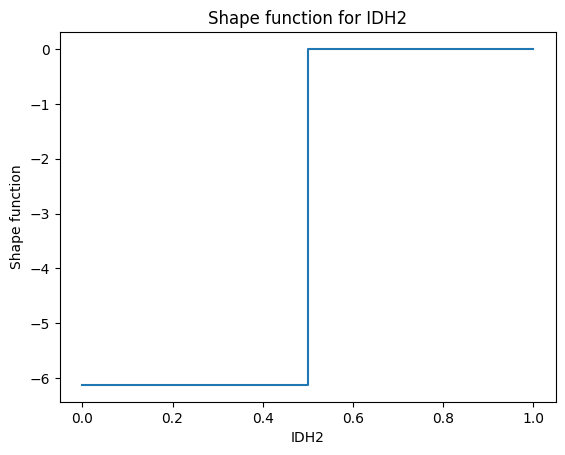
\includegraphics[width=0.3\textwidth]{idh2-shape.png}
  }
  \subfigure[NOTCH1]{
      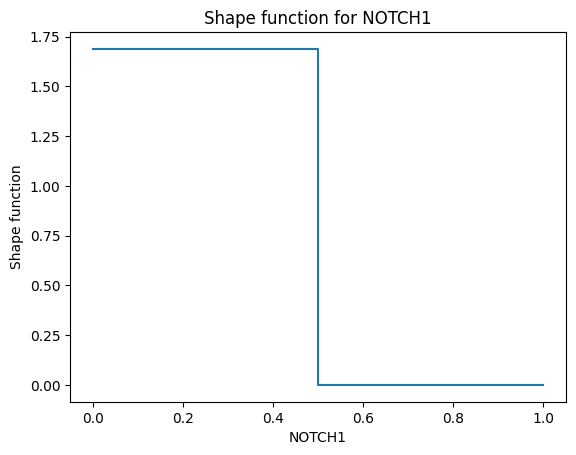
\includegraphics[width=0.3\textwidth]{notch1-shape.png}
  }
  \subfigure[PIK3R1]{
      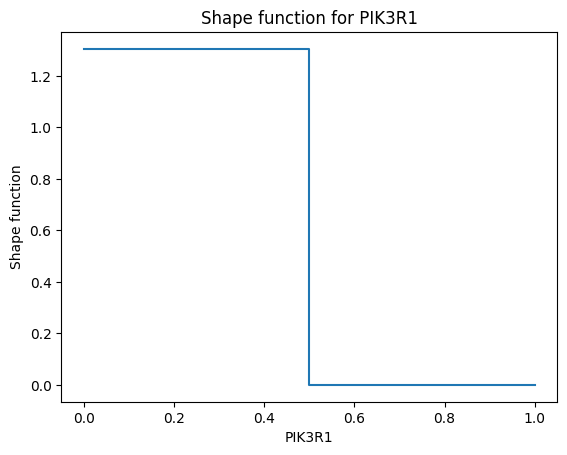
\includegraphics[width=0.3\textwidth]{pik3r1-shape.png}
  }
  \subfigure[TP53]{
    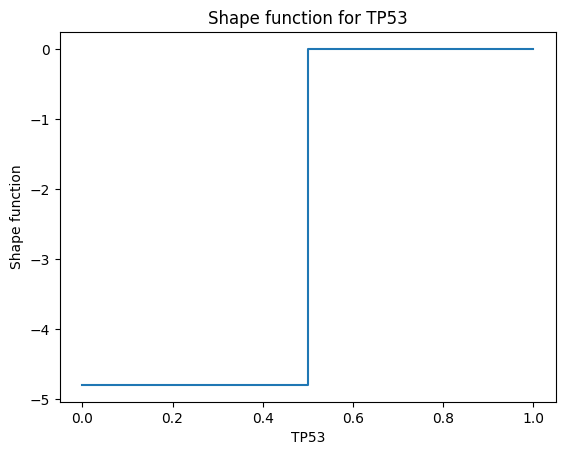
\includegraphics[width=0.3\textwidth]{TP53-shape.png}
  }
  \caption{Shape Functions for FastSparseGAM fit on training data, chosen to maximize balanced accuracy on test data.}
  \label{fig:shape}
\end{figure}

\begin{figure}[h!]
  \centering
  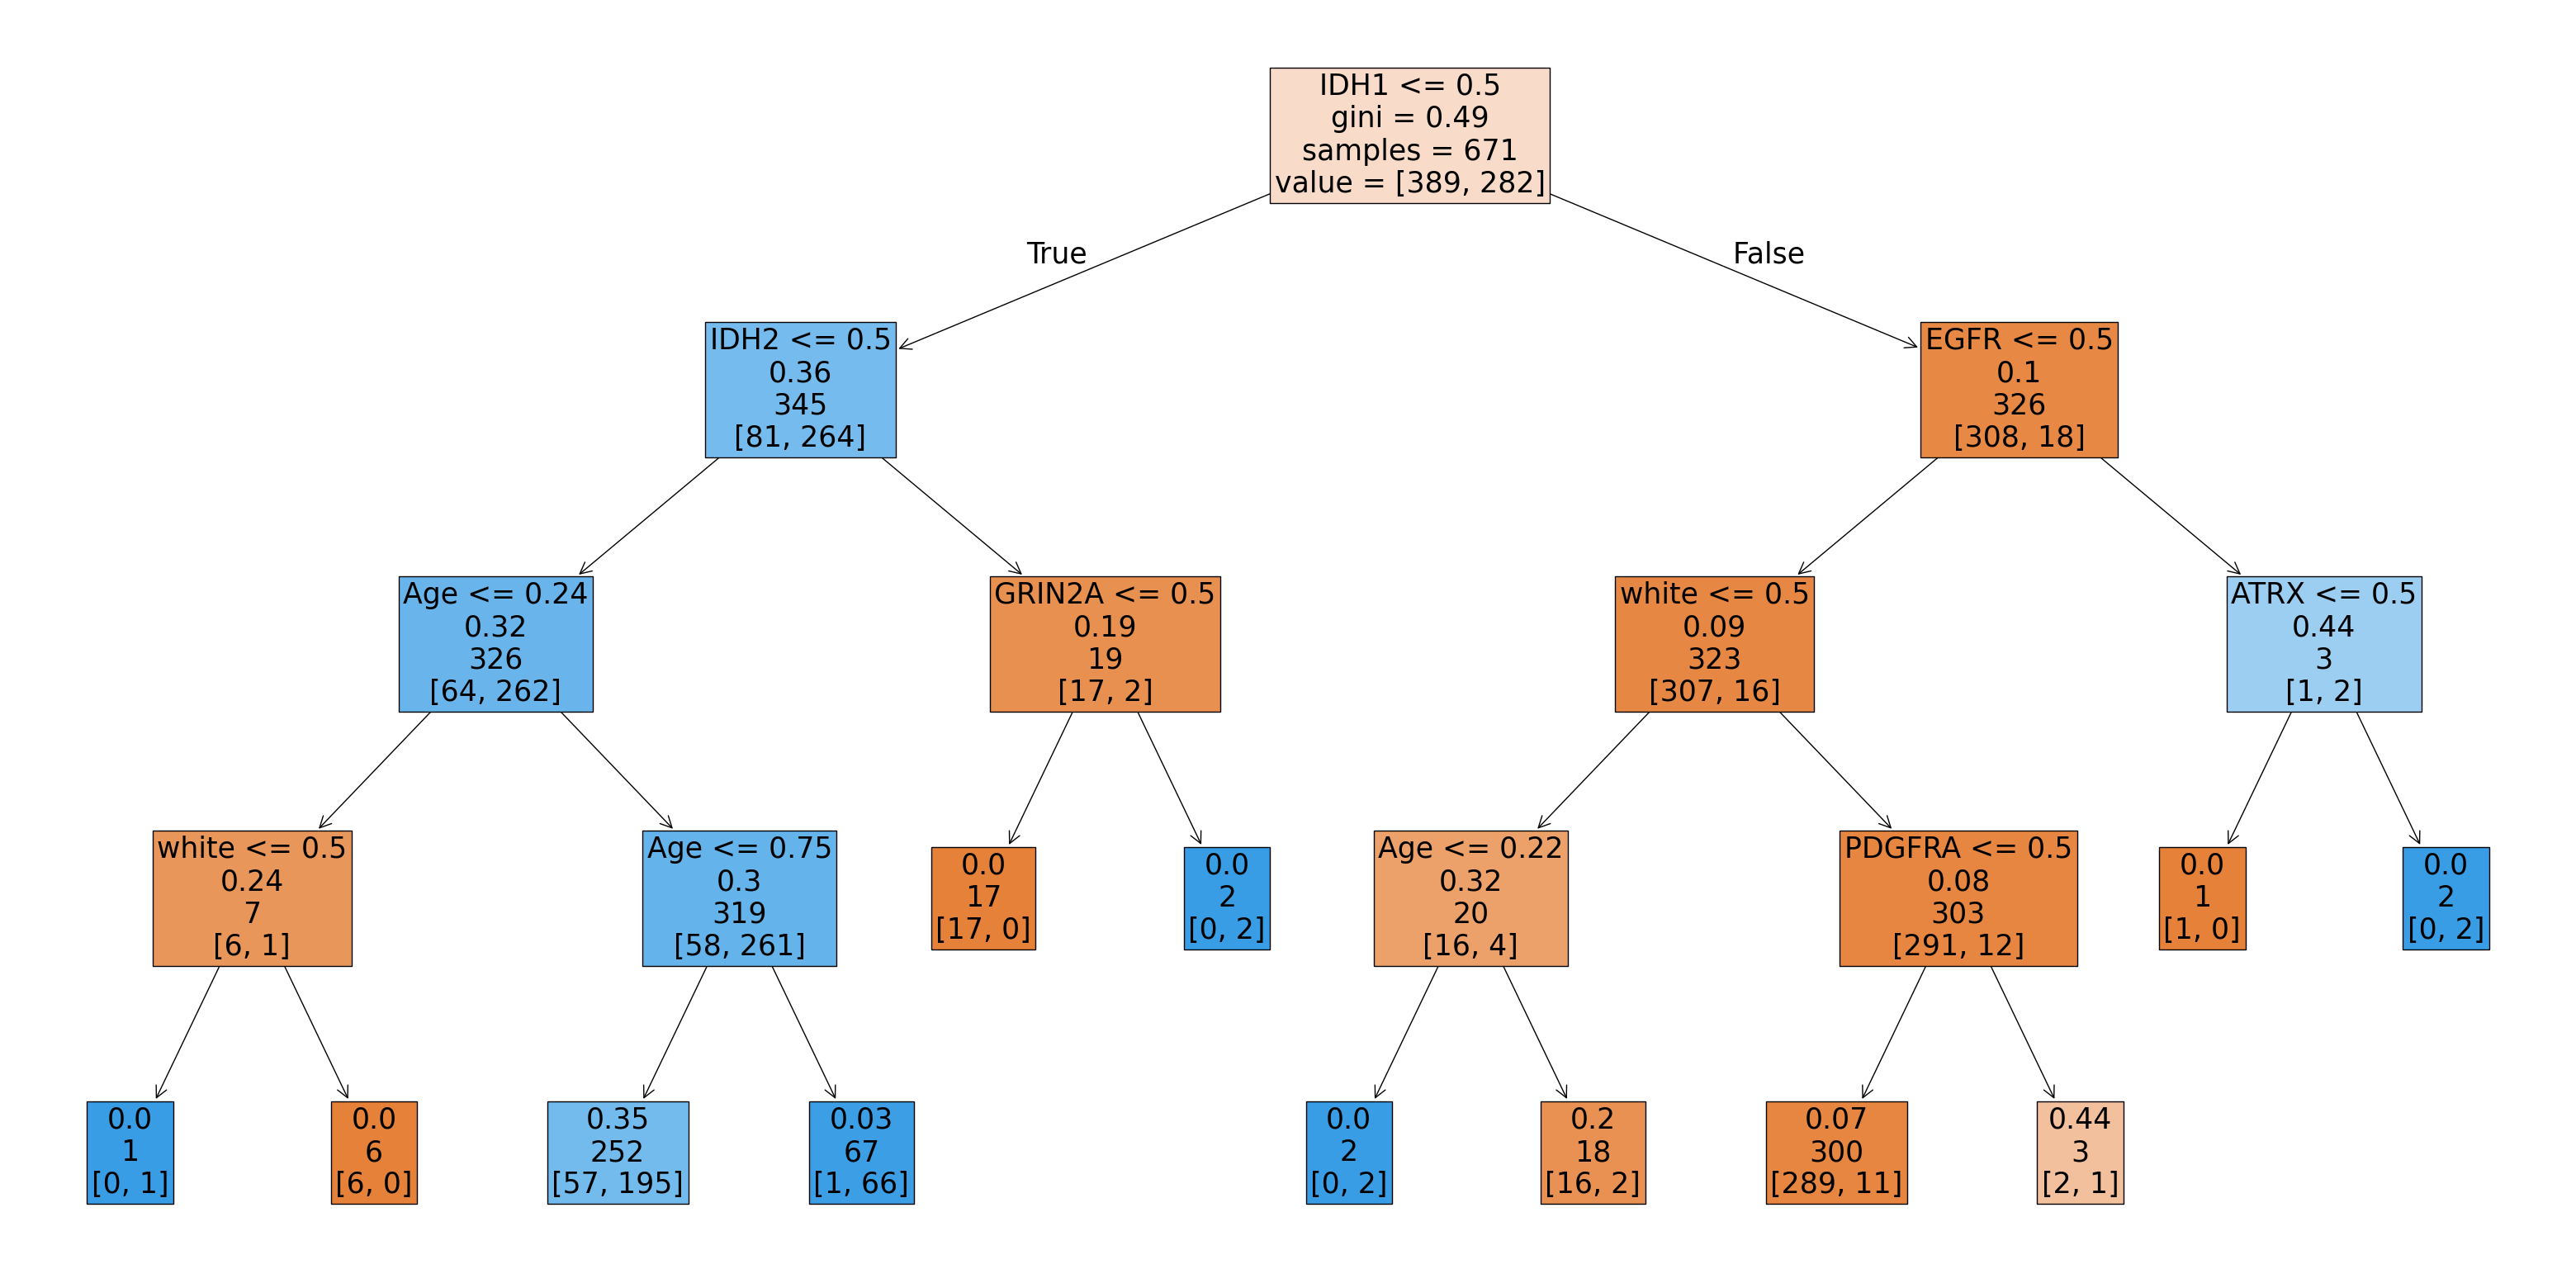
\includegraphics[scale = 0.2]{decision-tree.png}
  \caption{Decision tree trained on all of the training data}
  \label{fig:dtree-plot}
\end{figure}


\newpage
\section{Insight}
The interpretability of the models investigated in this report aligns well with exploratory data analysis and established biological findings regarding key markers that differentiate lower-grade gliomas (LGG) from glioblastoma multiforme (GBM). Among these, the mutation of IDH1 consistently emerges as the most significant marker across all models, exhibiting high variable importance scores. Additionally, age is identified as a critical factor, consistent with scientific literature indicating that GBM risk increases with age. These findings are robust across the range of models studied.

Despite these promising results, several issues persist with the TCGA glioma dataset. Notably, there is a lack of sufficient representation for certain feature levels. For example, the severe underrepresentation of American Indian and Alaska Native groups in the dataset is concerning. This imbalance complicates the ability of models to generalize and produce accurate predictions for these populations. This challenge is particularly pressing in healthcare, where underserved communities often experience disparities in treatment quality. Addressing the issue of small level sizes is essential for building models capable of making equitable and meaningful predictions.

Further improvements can be achieved by customizing loss functions to reflect real-world constraints and priorities. Conventional classification loss functions aim to reduce sparsity and misclassification errors but often neglect practical considerations such as cost and accessibility. For instance, as noted by Tasci et al., the IDH1 genetic test can be expensive and time-consuming. Incorporating data on the cost and efficiency of genetic tests into loss functions could lead to the identification of cost-effective combinations of tests with high predictive power. Expanding the dataset to include additional clinical features, such as histological information about tumor cell structure, may also enhance model performance.

The pursuit of interpretable yet optimal models remains an important focus. Techniques like generalized optimal sparse decision trees (GOSDT), which utilize bounds and dynamic programming to construct optimal and sparse trees, offer a promising avenue. Such models retain the interpretability of traditional decision trees while improving predictive performance and reducing complexity. Investigating similar sparse and interpretable models tailored to this domain may yield significant advancements.

Effective glioma grading hinges on the selection of relevant genetic markers, which can improve patient care and facilitate targeted drug and treatment discovery. Sparse and interpretable models empower healthcare providers to conduct tumor grading efficiently and cost-effectively, reducing the burden on patients. Addressing dataset limitations and enhancing model design with real-world considerations will further strengthen the quality of care for glioma patients and offer valuable insights into the biology of these tumors.


\section*{Citations}
Liu, J., Zhong, C., Seltzer, M., \& Rudin, C. (2022). Fast sparse classification for generalized linear and additive models. \textit{International Conference on Artificial Intelligence and Statistics}, 9304–9333. PMLR.

Pedregosa, F., Varoquaux, G., Gramfort, A., Michel, V., Thirion, B., Grisel, O., Blondel, M., Prettenhofer, P., Weiss, R., Dubourg, V., Vanderplas, J., Passos, A., Cournapeau, D., Brucher, M., Perrot, M., \& Duchesnay, E. (2011). Scikit-learn: Machine learning in Python. \textit{Journal of Machine Learning Research}, 12, 2825–2830.

Tasci, E., Camphausen, K., Krauze, A., \& Zhuge, Y. (2022). Glioma Grading Clinical and Mutation Features [Dataset]. UCI Machine Learning Repository. https://doi.org/10.24432/C5R62J.

\end{document}
